\documentclass[conference]{IEEEtran}
\IEEEoverridecommandlockouts
% The preceding line is only needed to identify funding in the first footnote. If that is unneeded, please comment it out.
\usepackage{matlab-prettifier}
\usepackage{cite}
\usepackage{amsmath,amssymb,amsfonts}
\usepackage{algorithmic}
\usepackage{graphicx}
\usepackage{textcomp}
\usepackage{xcolor}
\usepackage{float}
\def\BibTeX{{\rm B\kern-.05em{\sc i\kern-.025em b}\kern-.08em
    T\kern-.1667em\lower.7ex\hbox{E}\kern-.125emX}}

\begin{document}

\title{Project 3 : Importance Sampling}

\author{\IEEEauthorblockN{Owen Sowatzke}
\IEEEauthorblockA{\textit{Electrical Engineering Department} \\
\textit{University of Arizona}\\
Tucson, USA \\
osowatzke@arizona.edu}}
\maketitle

\begin{abstract}
Importance Sampling (IS) is an alternative to Monte Carlo (MC) simulation that can be used to estimate probabilities of hard-to-sample distributions. It more frequently samples the "important" samples of a distribution to reduce the variance of probability estimates. This document compares probabilities estimated with Monte Carlo Simulation and Importance Sampling. It specifically examines a case in which Monte Carlo Sampling provides very few "important" samples.
\end{abstract}

\begin{IEEEkeywords}
Monte Carlo Simulation, Importance Sampling,  Variance, Probability Estimates
\end{IEEEkeywords}

\section{Introduction}
Both Monte Carlo (MC) Simulations and Importance Sampling (IS) are techniques for estimating probabilities. In this document, both techniques will be used to estimate the probability that a random variable $X$ with distribution $X\sim N(1,1)$ exceeds 3.957 (i.e. $P\{X > 3.957\}$).
\section{Monte Carlo Simulation}
The probability of interest can be written as follows:
\begin{equation}
P\{X > 3.957\} = \int_{-\infty}^{\infty}I(x)f_X(x)dx
\end{equation}
where
\begin{equation}
I(x) = \begin{cases}
1 & x > 3.957 \\
0 & x \leq 3.957
\end{cases}
\end{equation}
Note that this probability can also be written as an expected value:
\begin{equation}
P\{X > 3.957\} = E[I(X)]
\end{equation}
Monte Carlo Simulation attempts to estimate this probability using a sample mean
\begin{equation}
P\{X > 3.957\} \approx \frac{1}{N}\sum_{i=1}^{N}I(x_i)
\end{equation}
where
\begin{equation}
x_1, x_2, ..., x_N \sim f_X(x)
\end{equation}
\par
Given different values of $N \in [1, 10^5]$, Monte Carlo Simulations can be used to estimate $P\{X > 3.957\}$. This estimate can than be compared to the true probability.
\begin{equation}
P\{X > 3.957\} = 0.001553
\end{equation}
The Monte Carlo probability estimate was generated for values $N$ from $100$ to $10^5$ in increments of $100$. The MATLAB code to generate this estimate is included in Appendix \ref{matlab_code}. The Monte Carlo probability estimate is plotted vs $N$ in Fig. \ref{Monte Carlo Estimate}
\begin{figure}[H]
\centerline{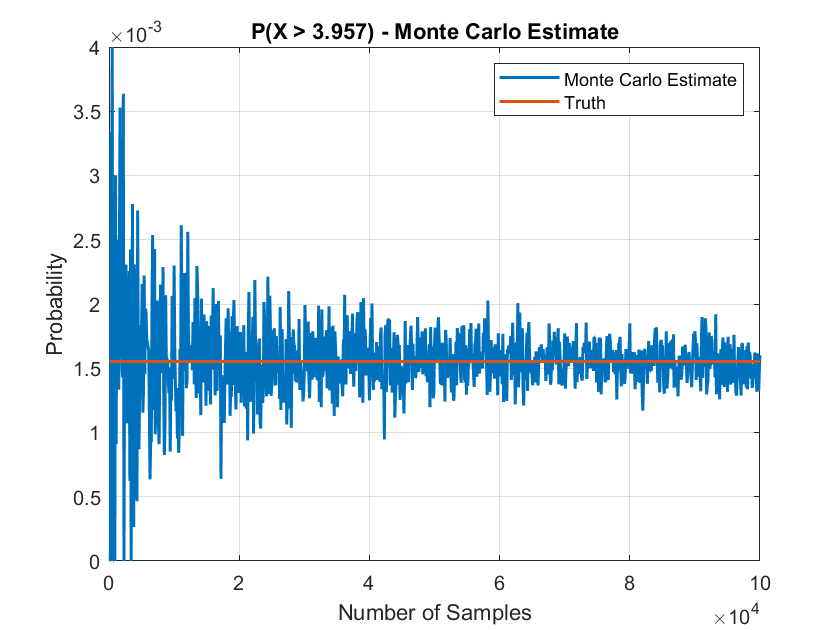
\includegraphics[width=0.5\textwidth]{Monte_Carlo_Estimate.png}}
\caption{Monte Carlo Probability Estimate}
\label{Monte Carlo Estimate}
\end{figure}
The absolute value of the error between the Monte Carlo estimate and the true probability ($|P_{est}\{X > 3.957\} - P_{truth}\{X > 3.957\}|$) is also plotted vs $N$.
\begin{figure}[H]
\centerline{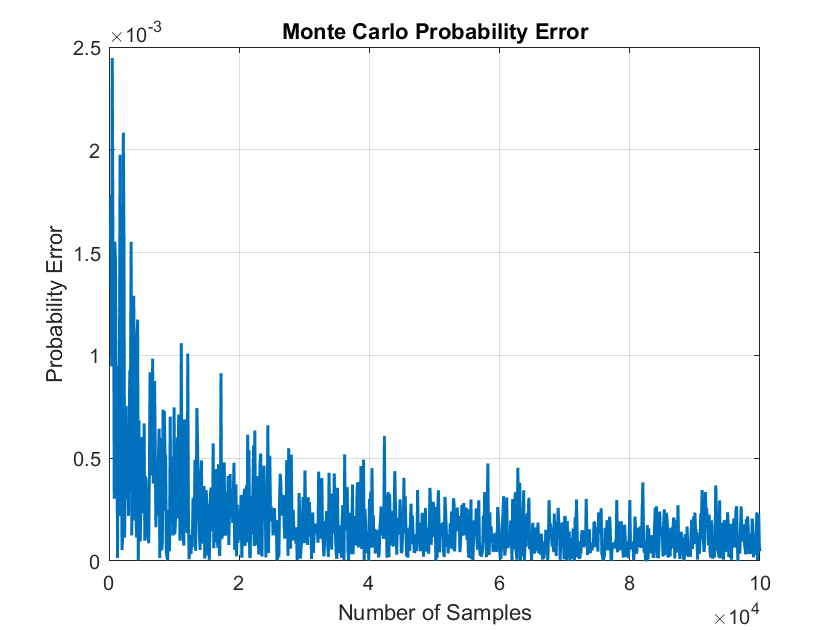
\includegraphics[width=0.5\textwidth]{Monte_Carlo_Error.png}}
\caption{Monte Carlo Probability Error}
\label{Monte Carlo PError}
\end{figure}

%both techniques will be used to estimate the following probability:
%\begin{equation}
%P\{X > 3.957\}
%\end{equation}
%will be used to compute the probability that a random variable $X$ exceeds a threshold $\lambda$.
%Let $X$ be a normally distributed distributed random variable with $\mu=1$ and $\sigma^2=1$ (i.e. $X \sim N(1,1)$). Next, consider $\lambda=3.957$. Now, both simulations methods will attempt to estimate $P\{X > 3.957\}$.
%Consider a pulsed radar system using threshold-based detection. The radar system transmits a signal and receives a return echo when a target is present. The receiver also receives Guassian-distributed thermal noise. If the received  signal sample is greater than the threshold, the radar detects a target. Conversely, if the received signal sample is smaller than the threshold, the radar does not detect a target. \par
%Let $H_1$ be an event that the target is present, and let $H_0$ be an event that the target is not present. Furthermore, define the signal return as a random variable $X$. The conditional densities of $X$ ($f_{X|H_0}(x|H_0)$ and $f_{X|H_1}(x|H_1)$) are Gaussian and centered about $\eta_0$ and $\eta_1$ respectively.
%\begin{equation}
%f_{X|H_0}(x|H_0)=\frac{1}{\sqrt{2\pi{\sigma}^2}}e^{-\frac{(x-\eta_0)^2}{2{\sigma}^2}}\label{general_f(x|H0)}
%\end{equation}
%\begin{equation}
%f_{X|H_1}(x|H_1)=\frac{1}{\sqrt{2\pi{\sigma}^2}}e^{-\frac{(x-\eta_1)^2}{2{\sigma}^2}}\label{general_f(x|H1)}
%\end{equation}
%The conditional densities of $X$ are illustrated in Fig. \ref{gen_cond_densities}.
%\begin{figure}[htbp]
%\centerline{\includegraphics[width=0.5\textwidth]{gen_cond_densities.png}}
%\caption{Conditional Densities of $X$.}
%\label{gen_cond_densities}
%\end{figure}
%\par
%As mentioned above, the received signal sample is compared to a threshold $\Lambda$ and is a decision is made about the target's presence. Let the event $D_1$ correspond to a detection (signal exceeds threshold) and $D_0$ correspond to no detection (signal does not exceed threshold). Decision regions for this scenario are shown in Fig. \ref{cond_decision_region}
%\begin{figure}[htbp]
%\centerline{\includegraphics[width=0.5\textwidth]{cond_decision_region.png}}
%\caption{Decision Regions Based on Threshold $\Lambda$.}
%\label{cond_decision_region}
%\end{figure}
%\par
%Two important probabilities for the radar system are probability of detection ($P_d$) and probability of false alarm ($P_{fa}$). Probability of detection is the probability a target is detected given that a target is present. Conversely, probability of false alarm is the probability a target is detected when there is no target. These probabilities are stated in equations \eqref{Pd_formula} and \eqref{Pfa_formula}.
%\begin{equation}
%P_d = P(\{X > \Lambda\}|H_1) = P(D_1|H_1) \label{Pd_formula}
%\end{equation}
%\begin{equation}
%P_{fa} = P(\{X > \Lambda\}|H_0) = P(D_1|H_0) \label{Pfa_formula}
%\end{equation}
%These probabilities are illustrated in Fig. \ref{pd_plot} and Fig. \ref{pfa_plot}.
%\begin{figure}[htbp]
%\centerline{\includegraphics[width=0.5\textwidth]{pd_plot.png}}
%\caption{Probability of Detection.}
%\label{pd_plot}
%\end{figure}
%\begin{figure}[htbp]
%\centerline{\includegraphics[width=0.5\textwidth]{pfa_plot.png}}
%\caption{Probability of False Alarm.}
%\label{pfa_plot}
%\end{figure}
%\par
%The radar system's threshold should be chosen to maximize the probability of detection and minimize the probability of false alarm. By decreasing the threshold $\Lambda$, the probability of detection can be increased. However, the probability of false alarm will also increase. Conversely, if the threshold $\Lambda$ is increased, both the probability of false alarm and the probability of detection will decrease. As such, there a tradeoffs to consider when selecting the threshold $\Lambda$.
%\par
%The Receiver Operating Characteristics (ROC) curve can be used to analyze these tradeoffs. It shows $P_d$ as a function of $P_{fa}$. This document derives the ROC curve for different values of SNR using analytic methods and Monte Carlo Simulations.
%\section{ROC Curve Derivation}
%\subsection{Refining the Problem}
%The Guassian noise received by the receiver is assumed to be zero-mean ($\eta_0 = 0$). The SNR of the system is given by equation \eqref{SNR_equation}.
%\begin{equation}
%SNR = 10log_{10}\frac{P_s}{P_n}\label{SNR_equation}
%\end{equation}
%Note that there are two ways to vary the SNR of the system. First, the power of the target return ($P_s$) can be increased while keeping the noise power ($P_n$) constant. Second, the noise power ($P_n$) can be increased while keeping the power of the target return ($P_s$) constant.
%\par
%The derivation that follows fixes the signal power, while varying the noise power. Assuming a constant amplitude target return, the power of the target return is given by equation \eqref{signal_power}.
%\begin{equation}
%P_s={\eta_1}^2\label{signal_power}
%\end{equation}
%For zero-mean Gaussian noise, the noise power is given by equation \eqref{noise_power}
%\begin{equation}
%P_s={\sigma}^2\label{noise_power}
%\end{equation}
%The signal power can be fixed at any positive non-zero value. For this derivation, it is fixed at 1. This results in $\eta_1=1$ and an SNR given by equation \eqref{SNR_simp}.
%\begin{equation}
%SNR = 10log_{10}\frac{1}{{\sigma}^2}\label{SNR_simp}
%\end{equation}
%\subsection{Analytic Derivation}
%With the assumptions given above, the conditional densities given in equations \eqref{general_f(x|H0)} and \eqref{general_f(x|H1)} can be rewritten as follows:
%\begin{equation}
%f_{X|H_0}(x|H_0)=\frac{1}{\sqrt{2\pi{\sigma}^2}}e^{-\frac{x^2}{2{\sigma}^2}}\label{specific_f(x|H0)}
%\end{equation}
%\begin{equation}
%f_{X|H_1}(x|H_1)=\frac{1}{\sqrt{2\pi{\sigma}^2}}e^{-\frac{(x-1)^2}{2{\sigma}^2}}\label{specific_f(x|H1)}
%\end{equation}
%\par
%The probability of detection is the area under $f_{X|H_1}(x|H_1)$ shown in Fig. \ref{pd_plot}. This area can be expressed by the integral given in equation \eqref{pd_int}.
%\begin{equation}
%P_d=\int_{\Lambda}^{\infty}f_{X|H_1}(x|H_1)dx\label{pd_int}
%\end{equation}
%Combining equations \eqref{specific_f(x|H1)} and \eqref{pd_int}, the probability of detection can be rewritten as follows:
%\begin{equation}
%P_d=\int_{\Lambda}^{\infty}\frac{1}{\sqrt{2\pi{\sigma}^2}}e^{-\frac{(x-1)^2}{2{\sigma}^2}}dx\label{pd_full_int}
%\end{equation}
%Note that this integral can be written in terms of the Q function, where the Q function is given below:
%\begin{equation}
%Q(x)=\frac{1}{\sqrt{2\pi}}\int_{x}^{\infty}e^{-\frac{t^2}{2}}dt\label{qfunc}
%\end{equation}
%To rewrite equation \eqref{pd_full_int} in terms of the Q function, define $t$ as follows:
%\begin{equation}
%t=\frac{x-1}{\sigma}
%\end{equation}
%$dx$ can now be rewritten in terms of $dt$.
%\begin{equation}
%dt=\frac{dx}{\sigma}
%\end{equation}
%\begin{equation}
%dx=\sigma dt
%\end{equation}
%The upper bound of the integral is still infinity and the lower bound of the integral is given by equation \eqref{pd_int_lower_bound}.
%\begin{equation}
%\frac{\Lambda-1}{\sigma}\label{pd_int_lower_bound}
%\end{equation}
%After substitution, $P_d$ can be expressed in the following form: 
%\begin{equation}
%P_d=\int_{\frac{\Lambda-1}{\sigma}}^{\infty}\frac{1}{\sqrt{2\pi{\sigma}^2}}e^{-\frac{t^2}{2}}\cdot \sigma dt 
%\label{pd_int_sub}
%\end{equation}
%Simplifying equation \eqref{pd_int_sub} leads to the following:
%\begin{equation}
%P_d=\int_{\frac{\Lambda-1}{\sigma}}^{\infty}\frac{1}{\sqrt{2\pi}}e^{-\frac{t^2}{2}}dt 
%\end{equation}
%\begin{equation}
%P_d=\frac{1}{\sqrt{2\pi}}\int_{\frac{\Lambda-1}{\sigma}}^{\infty}e^{-\frac{t^2}{2}}dt\label{pd_int_final}
%\end{equation}
%Note that equation \eqref{pd_int_final} is in the form of the Q function. $P_d$ can be expressed using the Q function as follows:
%\begin{equation}
%P_d = Q\left(\frac{\Lambda-1}{\sigma}\right)\label{pd_qfunc}
%\end{equation}
%\par
%The probability of false alarm can be derived in a similar manner. The probability of false alarm is the area under $f_{X|H_0}(x|H_0)$ shown in Fig. \ref{pfa_plot}. This area can be expressed by the integral given in equation \eqref{pfa_int}.
%\begin{equation}
%P_{fa}=\int_{\Lambda}^{\infty}f_{X|H_0}(x|H_0)dx\label{pfa_int}
%\end{equation}
%Combining equations \eqref{specific_f(x|H0)} and \eqref{pfa_int}, the probability of false alarm can be rewritten as follows:
%\begin{equation}
%P_{fa}=\int_{\Lambda}^{\infty}\frac{1}{\sqrt{2\pi{\sigma}^2}}e^{-\frac{x^2}{2{\sigma}^2}}dx\label{pfa_full_int}
%\end{equation}
%This integral can also be rewritten in terms of the Q function given by equation \eqref{qfunc}. To rewrite the integral, in terms of the Q function, define $t$ as follows:
%\begin{equation}
%t=\frac{x}{\sigma}
%\end{equation}
%$dx$ can now be rewritten in terms of $dt$.
%\begin{equation}
%dt=\frac{dx}{\sigma}
%\end{equation}
%\begin{equation}
%dx=\sigma dt
%\end{equation}
%The upper bound of the integral is still infinity and the lower bound of the integral is given by equation \eqref{pfa_int_lower_bound}.
%\begin{equation}
%\frac{\Lambda}{\sigma}\label{pfa_int_lower_bound}
%\end{equation}
%After substituion, $P_{fa}$ can be expressed in the following form:
%\begin{equation}
%P_{fa}=\int_{\frac{\Lambda}{\sigma}}^{\infty}\frac{1}{\sqrt{2\pi{\sigma}^2}}e^{-\frac{t^2}{2}}\cdot \sigma dt 
%\label{pfa_int_sub}
%\end{equation}
%Simplifying equation \eqref{pfa_int_sub} leads to the following:
%\begin{equation}
%P_{fa}=\int_{\frac{\Lambda}{\sigma}}^{\infty}\frac{1}{\sqrt{2\pi}}e^{-\frac{t^2}{2}}dt 
%\end{equation}
%\begin{equation}
%P_{fa}=\frac{1}{\sqrt{2\pi}}\int_{\frac{\Lambda}{\sigma}}^{\infty}e^{-\frac{t^2}{2}}dt\label{pfa_int_final}
%\end{equation}
%Note that equation \eqref{pfa_int_final} is in the form of the Q function. $P_{fa}$ can be expressed using the Q function as follows:
%\begin{equation}
%P_{fa} = Q\left(\frac{\Lambda}{\sigma}\right)\label{pfa_qfunc}
%\end{equation}
%\par
%Next, $P_d$ must be expressed in terms of $P_{fa}$. This is done by writing $\Lambda$ in terms of $P_{fa}$. 
%\begin{equation}
%\frac{\Lambda}{\sigma}=Q^{-1}(P_{fa})
%\label{lambda_conv_step1}
%\end{equation}
%\begin{equation}
%\Lambda=\sigma \cdot Q^{-1}(P_{fa})
%\label{lambda_conv_step2}
%\end{equation}
%Equations \eqref{lambda_conv_step2} and \eqref{pd_qfunc} can be combined to form the following:
%\begin{equation}
%P_d=Q\left(\frac{\sigma \cdot Q^{-1}(P_{fa}) - 1}{\sigma}\right)
%\end{equation}
%\begin{equation}
%P_d=Q\left(Q^{-1}(P_{fa})-\frac{1}{\sigma}\right)
%\label{pd_func_pfa}
%\end{equation}
%Equation \eqref{SNR_simp} can be used to express $\sigma$ in terms of SNR.
%\begin{equation}
%\frac{1}{\sigma^2}=10^{SNR/10}
%\end{equation}
%\begin{equation}
%\sigma^2=10^{-SNR/10}
%\end{equation}
%\begin{equation}
%\sigma=10^{-SNR/20}
%\label{sigma_func_SNR}
%\end{equation}
%Substituting $\sigma$ into equation \eqref{pd_func_pfa}, analytic ROC  curves can be generated for different values of SNR. The MATLAB code to perform this operation is included in Appendix \ref{analytic_code}, and the resulting ROC curve is shown in Fig. \ref{analytic_roc_curve}.
%\begin{figure}[htbp]
%\centerline{\includegraphics[width=0.5\textwidth]{Analytic_ROC_Curve.png}}
%\caption{Analytic ROC Curve.}
%\label{analytic_roc_curve}
%\end{figure}
%\subsection{Monte Carlo Derivation}
%The ROC curve can also be generated using Monte Carlo Simulations. This is done by taking a large number of samples of the random variable $X$ given $H_0$. These samples are compared to a threshold to determine the number of false alarms ($N_{fa}$). When the total number of samples ($N$) is large, the probability of false alarm is approximately given by the following:
%\begin{equation}
%P_{fa}\approx\frac{N_{fa}}{N}
%\end{equation}
%Similarly, a large number of samples of the random variable $X$ given $H_1$ can be taken. These samples are compared to a threshold to determine the number of detections ($N_d$). When the total number of samples ($N$) is large, the probability of detection is approximately given by the following:
%\begin{equation}
%P_d\approx\frac{N_d}{N}
%\end{equation}
%\par
%Each given threshold will provide one value of $P_d$ and one value of $P_{fa}$. This point is one sample on the ROC curve. Additional samples can be generated by sweeping through values of the threshold. This process can be repeated for each SNR to create a figure similar to Fig. \ref{analytic_roc_curve}. The MATLAB code for this operation is included in Appendix \ref{monte_carlo_code}, and the resulting ROC curve is shown in Fig. \ref{monte_carlo_roc_curve}.
%\begin{figure}[htbp]
%\centerline{\includegraphics[width=0.5\textwidth]{Monte_Carlo_ROC_Curve.png}}
%\caption{Monte Carlo ROC Curve.}
%\label{monte_carlo_roc_curve}
%\end{figure}
%\section{Conclusion}
%As illustrated in the ROC curves of Fig. \ref{analytic_roc_curve} and Fig. \ref{monte_carlo_roc_curve}, the analytic derivation of the ROC curve is approximately equivalent to curve produced using Monte Carlo Simulations. As such, the Monte Carlo simulations support the analytic results.
%\par
%Note that SNR also effects the shape of the ROC curves. Increased SNR moves the curve in Fig. \ref{analytic_roc_curve} and Fig. \ref{monte_carlo_roc_curve} towards the upper left corner of the plot. Therefore at increased SNR, it is possible to achieve higher probabilities of detection for a given probability of false alarm. This phenomenon can be explained as follows. Increased SNR will reduce the noise power and condense the conditional densities given in equations \eqref{specific_f(x|H0)} and \eqref{specific_f(x|H1)}. Examining Fig. \ref{pd_plot} and Fig. \ref{pfa_plot}, this will result in an increased probability of detection and decreased probability of false alarm. 
% This occurs because the reduction in the noise power condenses the conditional densities shown in Fig. \ref{gen_cond_densities}.
%\par 
%For a given SNR, the system designer can leverage the ROC curve to select a threshold that produces an optimal ratio between the probability of detection and probability of false alarm. This can be done by selecting a point on the ROC curve and mapping that point to a threshold using equation \eqref{lambda_conv_step2}. Using the methods illustrated in this document, ROC curves can be generated for other systems and leveraged when choosing their thresholds. % Finally, the ROC curves generated in this document are a very valuable tool for performing tradeoff analysis.
%For a given SNR, the system designer can select a point on the curve which produces a desired ratio between the probability of detection and probability of false alarm. This point can be mapped to the desired threshold using equation \eqref{lambda_conv_step2}. 

% The threshold used in the given radar system samples a point on the ROC curve. Choices of the threshold that maximize the probability of detection also increase the probability of false alarm. The derived ROC curve provides a method for selecting the optimal threshold for the system. To determine an optimal threshold the system designer can select an optimal point on the curve and compute the corresponding threshold using equation \eqref{lambda_conv_step2}.

\onecolumn
\pagebreak
\appendices
\section{MATLAB Source Code}
\label{matlab_code}
\lstset{style=Matlab-editor}
\lstinputlisting{Project3_Sowatzke.m}
\raggedbottom
%\pagebreak
%\section{MATLAB Code to Plot Monte Carlo ROC Curve}
%\label{monte_carlo_code}
%\lstset{style=Matlab-editor}
%\lstinputlisting{Monte_Carlo_ROC_Curve.m}
\end{document}
